\chapter{Arithmétique}
{https://sacado.xyz/qcm/parcours_show_course/0/117129}
{
 \begin{CpsCol}
\textbf{Les savoir-faire du parcours}
 \begin{itemize}
 \item Calculer une longueur dans un triangle
 \end{itemize}
 
 \end{CpsCol}
 
 \begin{His}
 
\begin{wrapfigure}[15]{r}{3.6cm}
\vspace{-7mm}
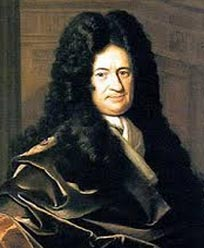
\includegraphics[scale=0.5]{FIG/liebniz.jpg}

\begin{center}
  \textsc{Thalès} de Milet \\
  né à Milet vers 625-620 av. J.-C. et mort vers 548-545 av. J.-C
 \end{center} 
\end{wrapfigure}

\textbf{\textsc{Thalès}} est d'abord commerçant et ingénieur mais aussi homme politique.

Grâce à son séjour en Égypte, Thalès put mettre en œuvre ses connaissances en mathématiques, particulièrement en géométrie, domaines dans lesquels il fit quelques découvertes fondamentales, comme déterminer qu'un cercle est partagé en deux parties égales par tout diamètre ou que les angles à la base d'un triangle isocèle sont égaux. 

Ses découvertes astronomiques permirent d'aider à la navigation en haute mer en repérant certaines étoiles ou en déterminant les éphémérides. Il est probable que Thalès ait consigné ses découvertes par écrit afin d'en diffuser l'utilité, même s'il ne demeure à ce jour aucun texte de sa main.

En Europe, le théorème de Thalès ne désigne pas la même chose. En Allemagne,le « théorème de Thalès » porte sur l'angle inscrit dans un demi-cercle : si un triangle est inscrit dans un cercle avec un côté du triangle pour diamètre du cercle, alors ce triangle est rectangle d'hypoténuse ce diamètre.

 \end{His}

}




\begin{pageCours}




\section{Le théorème de Thalès}


\begin{ThT}{Le théorème de Thalès}\index{Théorème de Thalès}

Soit $(AB)$ et $(CD)$ deux droites sécantes en $O$.
 
Si les droites $\left(AC\right)$ et $\left(BD\right)$ sont parallèles alors on a :$\dfrac{OA}{OB}=\dfrac{OC}{OD}=\dfrac{AC}{BD}$.

\vspace{0.4cm}

\begin{minipage}{0.48\linewidth}
\begin{center}
Configuration en voile

\begin{tikzpicture}[line cap=round,line join=round,>=triangle 45,x=1.0cm,y=1.0cm]
\clip(2.32,1.02) rectangle (7.04,4.22);
\draw [line width=1.pt,color=xdxdff] (3.3,2.36)-- (6.36,1.84);
\draw [line width=1.pt,color=xdxdff] (6.36,1.84)-- (5.,3.32);
\draw [line width=1.pt,color=xdxdff] (5.,3.32)-- (3.3,2.36);
\draw [line width=1.pt,color=xdxdff,domain=2.32:7.04] plot(\x,{(--0.844--0.96*\x)/1.7});
\draw [line width=1.pt,color=xdxdff,domain=2.32:7.04] plot(\x,{(--8.9376-0.52*\x)/3.06});
\draw [line width=1.pt,color=xdxdff] (5.09733655157939,2.0545702592087305)-- (4.298520306432994,2.923870290691573);
\begin{scriptsize}
\draw [color=ududff] (3.3,2.36)-- ++(-2.5pt,0 pt) -- ++(5.0pt,0 pt) ++(-2.5pt,-2.5pt) -- ++(0 pt,5.0pt);
\draw[color=ududff] (3.1,2.69) node {$O$};
\draw [color=ududff] (6.36,1.84)-- ++(-2.5pt,0 pt) -- ++(5.0pt,0 pt) ++(-2.5pt,-2.5pt) -- ++(0 pt,5.0pt);
\draw[color=ududff] (6.42,1.61) node {$D$};
\draw [color=ududff] (5.,3.32)-- ++(-2.5pt,0 pt) -- ++(5.0pt,0 pt) ++(-2.5pt,-2.5pt) -- ++(0 pt,5.0pt);
\draw[color=ududff] (5.14,3.69) node {$B$};
\draw [color=xdxdff] (4.298520306432994,2.923870290691573)-- ++(-2.5pt,0 pt) -- ++(5.0pt,0 pt) ++(-2.5pt,-2.5pt) -- ++(0 pt,5.0pt);
\draw[color=xdxdff] (4.2,3.37) node {$A$};
\draw [color=xdxdff] (5.09733655157939,2.0545702592087305)-- ++(-2.5pt,0 pt) -- ++(5.0pt,0 pt) ++(-2.5pt,-2.5pt) -- ++(0 pt,5.0pt);
\draw[color=xdxdff] (5.02,1.81) node {$C$};
\end{scriptsize}
\end{tikzpicture}
\end{center}
\end{minipage}
\hfill
\begin{minipage}{0.48\linewidth}
\begin{center}
Configuration en papillon

\begin{tikzpicture}[line cap=round,line join=round,>=triangle 45,x=1.0cm,y=1.0cm]
\clip(-0.38,-0.5) rectangle (4.56,2.48);
\draw [line width=1.pt,color=xdxdff] (1.48,0.92)-- (3.02,0.46);
\draw [line width=1.pt,color=xdxdff] (3.02,0.46)-- (3.98,1.98);
\draw [line width=1.pt,color=xdxdff] (3.98,1.98)-- (1.48,0.92);
\draw [line width=1.pt,color=xdxdff,domain=-0.38:4.56] plot(\x,{(--0.7312--1.06*\x)/2.5});
\draw [line width=1.pt,color=xdxdff,domain=-0.38:4.56] plot(\x,{(--2.0976-0.46*\x)/1.54});
\draw [line width=1.pt,color=xdxdff] (0.5133438211999565,1.2087414560052079)-- (-0.08924704350656398,0.2546392535532169);
\begin{scriptsize}
\draw [color=ududff] (1.48,0.92)-- ++(-2.5pt,0 pt) -- ++(5.0pt,0 pt) ++(-2.5pt,-2.5pt) -- ++(0 pt,5.0pt);
\draw[color=ududff] (1.28,1.25) node {$O$};
\draw [color=ududff] (3.02,0.46)-- ++(-2.5pt,0 pt) -- ++(5.0pt,0 pt) ++(-2.5pt,-2.5pt) -- ++(0 pt,5.0pt);
\draw[color=ududff] (2.98,0.03) node {$D$};
\draw [color=ududff] (3.98,1.98)-- ++(-2.5pt,0 pt) -- ++(5.0pt,0 pt) ++(-2.5pt,-2.5pt) -- ++(0 pt,5.0pt);
\draw[color=ududff] (4.12,2.35) node {$A$};
\draw [color=xdxdff] (-0.08924704350656398,0.2546392535532169)-- ++(-2.5pt,0 pt) -- ++(5.0pt,0 pt) ++(-2.5pt,-2.5pt) -- ++(0 pt,5.0pt);
\draw[color=xdxdff] (0.18,0.07) node {$B$};
\draw [color=xdxdff] (0.5133438211999565,1.2087414560052079)-- ++(-2.5pt,0 pt) -- ++(5.0pt,0 pt) ++(-2.5pt,-2.5pt) -- ++(0 pt,5.0pt);
\draw[color=xdxdff] (0.66,1.57) node {$C$};
\end{scriptsize}
\end{tikzpicture}
\end{center}
\end{minipage}
\end{ThT}




\begin{ExCor}

\begin{minipage}{8.cm}

Sur la figure ci-contre, $\left(AC \right)$ est parallèle à $\left(BD \right)$.

\begin{itemize}
\item  $OA = 6$ cm ;
\item  $OB = 10$ cm ;
\item  $OC = 8$ cm.
\end{itemize}

Calculer $OD$.

\vspace{0.2cm}
 
\end{minipage}
\begin{minipage}{8.cm}

\begin{tikzpicture}[line cap=round,line join=round,>=triangle 45,x=1.0cm,y=1.0cm]
\clip(1.36,1.22) rectangle (6.96,4.34);
\draw [line width=1.pt,color=xdxdff] (1.72,2.2)-- (6.36,1.84);
\draw [line width=1.pt,color=xdxdff] (6.36,1.84)-- (5.,3.32);
\draw [line width=1.pt,color=xdxdff] (5.,3.32)-- (1.72,2.2);
\draw [line width=1.pt,color=xdxdff,domain=1.36:6.96] plot(\x,{(--5.2896--1.12*\x)/3.28});
\draw [line width=1.pt,color=xdxdff,domain=1.36:6.96] plot(\x,{(--10.8272-0.36*\x)/4.64});
\draw [line width=1.pt,color=xdxdff] (4.445373071675939,1.9885486409906603)-- (3.6465568265295425,2.8578486724735024);
\begin{scriptsize}
\draw [color=ududff] (1.72,2.2)-- ++(-2.5pt,0 pt) -- ++(5.0pt,0 pt) ++(-2.5pt,-2.5pt) -- ++(0 pt,5.0pt);
\draw[color=ududff] (1.52,2.53) node {$O$};
\draw [color=ududff] (6.36,1.84)-- ++(-2.5pt,0 pt) -- ++(5.0pt,0 pt) ++(-2.5pt,-2.5pt) -- ++(0 pt,5.0pt);
\draw[color=ududff] (6.42,1.61) node {$D$};
\draw [color=ududff] (5.,3.32)-- ++(-2.5pt,0 pt) -- ++(5.0pt,0 pt) ++(-2.5pt,-2.5pt) -- ++(0 pt,5.0pt);
\draw[color=ududff] (5.14,3.69) node {$B$};
\draw[color=xdxdff] (-4.08,0.55) node {$f$};
\draw[color=xdxdff] (-4.08,2.51) node {$g$};
\draw [color=xdxdff] (3.6465568265295425,2.8578486724735024)-- ++(-2.5pt,0 pt) -- ++(5.0pt,0 pt) ++(-2.5pt,-2.5pt) -- ++(0 pt,5.0pt);
\draw[color=xdxdff] (3.54,3.31) node {$A$};
\draw [color=xdxdff] (4.445373071675939,1.9885486409906603)-- ++(-2.5pt,0 pt) -- ++(5.0pt,0 pt) ++(-2.5pt,-2.5pt) -- ++(0 pt,5.0pt);
\draw[color=xdxdff] (4.36,1.73) node {$C$};
\end{scriptsize}
\end{tikzpicture}

\end{minipage}
\begin{minipage}{1.5cm}
\colorbox{sacado_blue}{\miniqr{1234}}
\end{minipage}
 
\begin{minipage}{10cm}
\begin{itemize}[leftmargin=*]
\item Les droites $(AB)$ et $(CD)$ sont sécantes en $O$. 
\item La droite $\left(AC \right)$ est parallèle à $\left( BD \right)$
\end{itemize}
\end{minipage}
\begin{minipage}{8cm}
 {\color{sacado_blue}\textbf{[1. Contexte de la situation]}}
\end{minipage}

\vspace{0.1cm}

Donc, d'après le théorème de Thalès, $\frac{OA}{OB}=\frac{OC}{OD}=\frac{AC}{BD}$ {\color{sacado_blue}\textbf{[2. Écrire les égalités des trois quotients]}}

Donc $\dfrac{6}{10}=\dfrac{8}{OD}=\dfrac{AC}{BD}$ {\color{sacado_blue}\textbf{[3. Remplacer les valeurs connues]}}

Comme $\dfrac{6}{10}=\dfrac{8}{OD}$ {\color{sacado_blue}\textbf{[4. Conserver généralement une seule égalité]}}

On déduit que $6\times OD=8 \times 10$ {\color{sacado_blue}\textbf{[5. Écrire de l'égalité à partir du produit en croix]}}

$OD= \dfrac{8 \times 10}{6}= \dfrac{8 \times 5}{3}= \dfrac{40}{3}$  (on \og isole \fg{} la longueur cherchée) et donc $OD=\dfrac{40}{3}$ cm {\color{sacado_blue}\textbf{[6. Conclure]}}.
\end{ExCor}











\begin{ExCor}

\begin{minipage}{8.cm}

Sur la figure ci-contre, $\left(YT\right)$ est parallèle à $\left(OJ\right)$.

\begin{itemize}
\item  $RT = 3$ cm ;
\item  $RO = 5$ cm ;
\item  $RY = 4,5$ cm.
\end{itemize}

Calculer $RJ$.

\vspace{0.2cm}
 
\end{minipage}
\begin{minipage}{8.cm}

\begin{tikzpicture}[line cap=round,line join=round,>=triangle 45,x=1.0cm,y=1.0cm]
\clip(0.1,0.74) rectangle (6.58,4.04);
\draw [line width=1.pt,color=xdxdff] (3.3,2.36)-- (5.66,1.74);
\draw [line width=1.pt,color=xdxdff] (5.66,1.74)-- (5.,3.32);
\draw [line width=1.pt,color=xdxdff] (5.,3.32)-- (3.3,2.36);
\draw [line width=1.pt,color=xdxdff,domain=0.1:6.58] plot(\x,{(--0.844--0.96*\x)/1.7});
\draw [line width=1.pt,color=xdxdff,domain=0.1:6.58] plot(\x,{(--7.6156-0.62*\x)/2.36});
\draw [line width=1.pt,color=xdxdff] (0.8507670608657913,3.003442551806444)-- (1.5357220353694259,1.3637018552674407);
\begin{scriptsize}
\draw [color=xdxdff] (3.3,2.36)-- ++(-2.5pt,0 pt) -- ++(5.0pt,0 pt) ++(-2.5pt,-2.5pt) -- ++(0 pt,5.0pt);
\draw[color=xdxdff] (3.1,2.69) node {$R$};
\draw [color=xdxdff] (5.66,1.74)-- ++(-2.5pt,0 pt) -- ++(5.0pt,0 pt) ++(-2.5pt,-2.5pt) -- ++(0 pt,5.0pt);
\draw[color=xdxdff] (5.62,1.31) node {$Y$};
\draw [color=xdxdff] (5.,3.32)-- ++(-2.5pt,0 pt) -- ++(5.0pt,0 pt) ++(-2.5pt,-2.5pt) -- ++(0 pt,5.0pt);
\draw[color=xdxdff] (5.14,3.69) node {$T$};
\draw [color=xdxdff] (1.5357220353694259,1.3637018552674407)-- ++(-2.5pt,0 pt) -- ++(5.0pt,0 pt) ++(-2.5pt,-2.5pt) -- ++(0 pt,5.0pt);
\draw[color=xdxdff] (1.8,1.17) node {$O$};
\draw [color=xdxdff] (0.8507670608657913,3.003442551806444)-- ++(-2.5pt,0 pt) -- ++(5.0pt,0 pt) ++(-2.5pt,-2.5pt) -- ++(0 pt,5.0pt);
\draw[color=xdxdff] (0.76,3.39) node {$J$};
\end{scriptsize}
\end{tikzpicture}

\end{minipage}
\begin{minipage}{1.5cm}
\colorbox{sacado_blue}{\miniqr{1234}}
\end{minipage}
 
\begin{minipage}{10cm}
\begin{itemize}[leftmargin=*]
\item Les droites $(JY)$ et $(OT)$ sont sécantes en $R$. 
\item La droite $\left(YT\right)$ est parallèle à $\left(OJ\right)$
\end{itemize}
\end{minipage}
\begin{minipage}{8cm}
 {\color{sacado_blue}\textbf{[1. Contexte de la situation]}}
\end{minipage}

\vspace{0.1cm}

Donc, d'après le théorème de Thalès, $\dfrac{RY}{RJ}=\dfrac{RT}{RO}=\dfrac{YT}{JO}$ {\color{sacado_blue}\textbf{[2. Écrire les égalités des trois quotients]}}

Donc $\dfrac{4,5}{RJ}=\dfrac{3}{5}=\dfrac{YT}{JO}$ {\color{sacado_blue}\textbf{[3. Remplacer les valeurs connues]}}

Donc $\dfrac{4,5}{RJ}=\dfrac{3}{5}$ {\color{sacado_blue}\textbf{[4. Conserver généralement une seule égalité]}}

On déduit que $4,5 \times 5=3\times RJ$ {\color{sacado_blue}\textbf{[5. Écrire de l'égalité à partir du produit en croix]}}

$RJ= \dfrac{4,5 \times 5}{3}$  (on \og isole \fg{} la longueur cherchée) et donc $RJ=7,5$ cm {\color{sacado_blue}\textbf{[6. Conclure]}}.
\end{ExCor}


\end{pageCours} 
\begin{pageAD} 
 

\Sf{Reconnaitre une situation de Thalès.}
 
\begin{ExoCad}{Modéliser. Calculer.}{1234}{0}{0}{0}{0}{0}

Écrire le théorème de Thalès associé à chaque configuration.

\begin{minipage}{0.48\linewidth}

\definecolor{xdxdff}{rgb}{0.49019607843137253,0.49019607843137253,1.}
\definecolor{qqqqff}{rgb}{0.,0.,1.}
\definecolor{ududff}{rgb}{0.30196078431372547,0.30196078431372547,1.}
\begin{tikzpicture}[line cap=round,line join=round,>=triangle 45,x=1.0cm,y=1.0cm]
\clip(0.14,0.5) rectangle (6.04,4.5);
\draw [line width=1.pt,color=xdxdff] (1.,1.)-- (5.4,1.18);
\draw [line width=1.pt,color=xdxdff] (5.4,1.18)-- (3.98,3.78);
\draw [line width=1.pt,color=xdxdff] (3.98,3.78)-- (1.,1.);
\draw [line width=1.pt,color=xdxdff] (2.8840981002867094,2.7576485633547154)-- (3.7818898125038674,1.1138045832387946);
\begin{scriptsize}
\draw [color=xdxdff] (1.,1.)-- ++(-2.5pt,0 pt) -- ++(5.0pt,0 pt) ++(-2.5pt,-2.5pt) -- ++(0 pt,5.0pt);
\draw[color=xdxdff] (0.8,1.33) node {$A$};
\draw [color=xdxdff] (5.4,1.18)-- ++(-2.5pt,0 pt) -- ++(5.0pt,0 pt) ++(-2.5pt,-2.5pt) -- ++(0 pt,5.0pt);
\draw[color=xdxdff] (5.64,1.21) node {$B$};
\draw [color=xdxdff] (3.98,3.78)-- ++(-2.5pt,0 pt) -- ++(5.0pt,0 pt) ++(-2.5pt,-2.5pt) -- ++(0 pt,5.0pt);
\draw[color=xdxdff] (4.12,4.15) node {$C$};
\draw [color=xdxdff] (3.7818898125038674,1.1138045832387946)-- ++(-2.5pt,0 pt) -- ++(5.0pt,0 pt) ++(-2.5pt,-2.5pt) -- ++(0 pt,5.0pt);
\draw[color=xdxdff] (4.08,0.91) node {$D$};
\draw [color=qqqqff] (2.8840981002867094,2.7576485633547154)-- ++(-2.0pt,0 pt) -- ++(4.0pt,0 pt) ++(-2.0pt,-2.0pt) -- ++(0 pt,4.0pt);
\draw[color=qqqqff] (3.,3.23) node {$E$};
\end{scriptsize}
\end{tikzpicture}

\point{6}
\end{minipage}
\hfill
\begin{minipage}{0.48\linewidth}

\definecolor{xdxdff}{rgb}{0.49019607843137253,0.49019607843137253,1.}
\definecolor{qqqqff}{rgb}{0.,0.,1.}
\definecolor{ududff}{rgb}{0.30196078431372547,0.30196078431372547,1.}
\begin{tikzpicture}[line cap=round,line join=round,>=triangle 45,x=1.0cm,y=1.0cm]
\clip(-1.08,-0.56) rectangle (5.42,2.52);
\draw [line width=1.pt,color=xdxdff] (1.48,0.92)-- (4.76,0.3);
\draw [line width=1.pt,color=xdxdff] (4.76,0.3)-- (3.98,1.98);
\draw [line width=1.pt,color=xdxdff] (3.98,1.98)-- (1.48,0.92);
\draw [line width=1.pt,color=xdxdff,domain=-1.08:5.42] plot(\x,{(--0.7312--1.06*\x)/2.5});
\draw [line width=1.pt,color=xdxdff,domain=-1.08:5.42] plot(\x,{(--3.9352-0.62*\x)/3.28});
\draw [line width=1.pt,color=xdxdff] (-0.5788521210806118,1.3091732667896279)-- (-0.08924704350656393,0.2546392535532168);
\begin{scriptsize}
\draw [color=xdxdff] (1.48,0.92)-- ++(-2.5pt,0 pt) -- ++(5.0pt,0 pt) ++(-2.5pt,-2.5pt) -- ++(0 pt,5.0pt);
\draw[color=xdxdff] (1.28,1.25) node {$A$};
\draw [color=xdxdff] (4.76,0.3)-- ++(-2.5pt,0 pt) -- ++(5.0pt,0 pt) ++(-2.5pt,-2.5pt) -- ++(0 pt,5.0pt);
\draw[color=xdxdff] (4.72,-0.13) node {$B$};
\draw [color=xdxdff] (3.98,1.98)-- ++(-2.5pt,0 pt) -- ++(5.0pt,0 pt) ++(-2.5pt,-2.5pt) -- ++(0 pt,5.0pt);
\draw[color=xdxdff] (4.12,2.35) node {$C$};
\draw [color=xdxdff] (-0.08924704350656393,0.2546392535532168)-- ++(-2.5pt,0 pt) -- ++(5.0pt,0 pt) ++(-2.5pt,-2.5pt) -- ++(0 pt,5.0pt);
\draw[color=xdxdff] (0.18,0.07) node {$D$};
\draw [color=xdxdff] (-0.5788521210806118,1.3091732667896279)-- ++(-2.5pt,0 pt) -- ++(5.0pt,0 pt) ++(-2.5pt,-2.5pt) -- ++(0 pt,5.0pt);
\draw[color=xdxdff] (-0.44,1.67) node {$E$};
\end{scriptsize}
\end{tikzpicture}


\point{6}
\end{minipage}


\end{ExoCad}

 
\Sf{Calculer une longueur avec le théorème de Thalès.}

\begin{ExoCad}{Calculer.}{1234}{0}{0}{0}{0}{0}


\begin{minipage}{0.48\linewidth}

\definecolor{xdxdff}{rgb}{0.49019607843137253,0.49019607843137253,1.}
\definecolor{qqqqff}{rgb}{0.,0.,1.}
\definecolor{ududff}{rgb}{0.30196078431372547,0.30196078431372547,1.}
\begin{tikzpicture}[line cap=round,line join=round,>=triangle 45,x=1.0cm,y=1.0cm]
\clip(0.14,0.5) rectangle (6.04,4.5);
\draw [line width=1.pt,color=xdxdff] (1.,1.)-- (5.4,1.18);
\draw [line width=1.pt,color=xdxdff] (5.4,1.18)-- (3.98,3.78);
\draw [line width=1.pt,color=xdxdff] (3.98,3.78)-- (1.,1.);
\draw [line width=1.pt,color=xdxdff] (2.8840981002867094,2.7576485633547154)-- (3.7818898125038674,1.1138045832387946);
\begin{scriptsize}
\draw [color=xdxdff] (1.,1.)-- ++(-2.5pt,0 pt) -- ++(5.0pt,0 pt) ++(-2.5pt,-2.5pt) -- ++(0 pt,5.0pt);
\draw[color=xdxdff] (0.8,1.33) node {$R$};
\draw [color=xdxdff] (5.4,1.18)-- ++(-2.5pt,0 pt) -- ++(5.0pt,0 pt) ++(-2.5pt,-2.5pt) -- ++(0 pt,5.0pt);
\draw[color=xdxdff] (5.64,1.21) node {$A$};
\draw [color=xdxdff] (3.98,3.78)-- ++(-2.5pt,0 pt) -- ++(5.0pt,0 pt) ++(-2.5pt,-2.5pt) -- ++(0 pt,5.0pt);
\draw[color=xdxdff] (4.12,4.15) node {$T$};
\draw [color=xdxdff] (3.7818898125038674,1.1138045832387946)-- ++(-2.5pt,0 pt) -- ++(5.0pt,0 pt) ++(-2.5pt,-2.5pt) -- ++(0 pt,5.0pt);
\draw[color=xdxdff] (4.08,0.91) node {$I$};
\draw [color=qqqqff] (2.8840981002867094,2.7576485633547154)-- ++(-2.0pt,0 pt) -- ++(4.0pt,0 pt) ++(-2.0pt,-2.0pt) -- ++(0 pt,4.0pt);
\draw[color=qqqqff] (3.,3.23) node {$Z$};
\end{scriptsize}
\end{tikzpicture}

Les droites $(AT)$ et $(IZ)$ sont parallèles. $RA=8$, 

$RI=5$, $AT=7$. 

Calculer $IZ$.
\end{minipage}
\begin{minipage}{0.48\linewidth}
\point{10}
\end{minipage}
\end{ExoCad}



\begin{ExoCad}{Calculer.}{1234}{0}{0}{0}{0}{0}
 
\begin{minipage}{0.48\linewidth}
\begin{tikzpicture}[line cap=round,line join=round,>=triangle 45,x=1.0cm,y=1.0cm]
\clip(0.06,1.26) rectangle (6.92,4.88);
\draw [line width=1.pt,color=xdxdff] (3.12,3.02)-- (5.28,2.14);
\draw [line width=1.pt,color=xdxdff] (5.28,2.14)-- (6.4,4.14);
\draw [line width=1.pt,color=xdxdff] (6.4,4.14)-- (3.12,3.02);
\draw [line width=1.pt,color=xdxdff,domain=0.06:6.92] plot(\x,{(--6.4112--1.12*\x)/3.28});
\draw [line width=1.pt,color=xdxdff,domain=0.06:6.92] plot(\x,{(--9.2688-0.88*\x)/2.16});
\draw [line width=1.pt,color=xdxdff] (1.508630793819925,3.676483750665956)-- (0.6731060202450717,2.184475226425147);
\begin{scriptsize}
\draw [color=ududff] (3.12,3.02)-- ++(-2.5pt,0 pt) -- ++(5.0pt,0 pt) ++(-2.5pt,-2.5pt) -- ++(0 pt,5.0pt);
\draw[color=ududff] (2.92,3.35) node {$A$};
\draw [color=ududff] (5.28,2.14)-- ++(-2.5pt,0 pt) -- ++(5.0pt,0 pt) ++(-2.5pt,-2.5pt) -- ++(0 pt,5.0pt);
\draw[color=ududff] (5.34,1.91) node {$V$};
\draw [color=ududff] (6.4,4.14)-- ++(-2.5pt,0 pt) -- ++(5.0pt,0 pt) ++(-2.5pt,-2.5pt) -- ++(0 pt,5.0pt);
\draw[color=ududff] (6.54,4.51) node {$E$};
\draw [color=xdxdff] (0.6731060202450717,2.184475226425147)-- ++(-2.5pt,0 pt) -- ++(5.0pt,0 pt) ++(-2.5pt,-2.5pt) -- ++(0 pt,5.0pt);
\draw[color=xdxdff] (0.58,2.63) node {$U$};
\draw [color=xdxdff] (1.508630793819925,3.676483750665956)-- ++(-2.5pt,0 pt) -- ++(5.0pt,0 pt) ++(-2.5pt,-2.5pt) -- ++(0 pt,5.0pt);
\draw[color=xdxdff] (1.52,4.13) node {$C$};
\end{scriptsize}
\end{tikzpicture}
 
 
 Les droites $(UC)$ et $(EV)$ sont parallèles. 
 
 $CA=5$cm, $CU=6$cm, $AV=7$cm. 

Calculer $EV$.
\end{minipage}
\begin{minipage}{0.48\linewidth}
\point{10}
\end{minipage}
\end{ExoCad}

 




\end{pageAD}

\begin{pageCours}

\section{Agrandissement et Réduction}

\begin{DefT}{Agrandissement et Réduction}\index{Agrandissement}\index{Réduction}
Si	deux figures ont la même forme et des longueurs proportionnelles, 
alors on dit que l'une est un \textbf{agrandissement ou une réduction} de l'autre.
\end{DefT}

\begin{Rq}
Le coefficient de proportionnalité $k$ est le rapport d'agrandissement ou de réduction.
\end{Rq}

\begin{Rq} 
\begin{itemize}[leftmargin=*]
\item  Les dimensions du triangle $OAC$ sont proportionnelles aux dimensions du triangle $OBD$.
\item  Le coefficient de proportionnalité est $\dfrac{OA}{OB}$ ou $\dfrac{OC}{OD}$ ou encore $\dfrac{AC}{BD}$. Lorsque ce rapport est supérieur à 1, on parle d'\textbf{agrandissement} sinon on parle de \textbf{réduction}.
\item  Dans ces configurations, on dit que les triangles sont \textbf{semblables}.\index{Triangles semblables}
\end{itemize}
\end{Rq}


\begin{ExCor}

\begin{minipage}{0.48\linewidth}
Le triangle $ABC$ a les dimensions suivantes.
\\$AB = 1,5$ cm
\\$BC = 2,5$ cm
\\$AC = 3,2$ cm

$DEF$ est un agrandissement de $ABC$ de rapport $1,6$. 

Calculer le périmètre $\mathcal{P}$ du triangle $DEF$.
\end{minipage}
\begin{minipage}{0.48\linewidth}
$DE = 1,6 \times AB = 1,6 \times 1,5 = 2,4$ cm

$DF = 1,6 \times AC = 1,6 \times 2,5 = 4$ cm

$EF = 1,6 \times BC = 1,6 \times 3,2 = 5,12$ cm

$\mathcal{P} = 2,4 + 4 + 5,12 = 11,52 (= 1,6 \times 7,2) $cm
\end{minipage}

\end{ExCor}

\begin{Rq} 
\begin{itemize}
\item $ABC$ est une réduction de $DEF$ de rapport $\dfrac{1,5}{2,4}  = \dfrac{2,5}{4} =\dfrac{3,2}{5,12}  = 0,625$.
\item Dans un agrandissement ou une réduction, les mesures des angles, la perpendicularité 
et le parallélisme sont conservés.
\end{itemize}
\end{Rq}



\begin{ThT}{Rapport d'agrandissement et/ou de réduction}\index{Rapport d'aires}\index{Rapport de volumes}
Si $k$ est le rapport de proportion de longueur alors :
\begin{itemize}[leftmargin=*]
\item  les aires sont multipliées par $k^2$.
\item  les volumes sont multipliés par $k^3$.
\end{itemize}
\end{ThT}




\end{pageCours} 
\begin{pageAD} 
 
\Sf{Calculer un coefficient d'agrandissement ou de réduction.}


\begin{ExoCad}{Calculer.}{1234}{0}{0}{0}{0}{0}

 

\end{ExoCad}



\end{pageAD}
%%%%%%%%%%%%%%%%%%%%%%%%%%%%%%%%%%%%%%%%%%%%%%%%%%%%%%%%%%%%%%%%%%%
%%%%  Niveau 1
%%%%%%%%%%%%%%%%%%%%%%%%%%%%%%%%%%%%%%%%%%%%%%%%%%%%%%%%%%%%%%%%%%%
\begin{pageParcoursu} 

 %%%%%%%%%%%%%%%%%%%%%%%%%%%
 

\begin{ExoCu}{Communiquer.}{1234}{0}{0}{0}{0}{0}

Soit $EFGH$ un parallélogramme tel que $EF=4$~cm; $FH=5$~cm et
$EH=6$~cm. \\Soit $K$ le point du segment $[EH]$ tel que
$HK=1,2$~cm.\\La parallèle à la droite $(EF)$ passant par $K$ coupe le
segment $[FH]$ en $J$.\par Calculer les longueurs $HJ$ et $JK$.

\end{ExoCu}


\begin{ExoCu}{Communiquer.}{1234}{0}{0}{0}{0}{0}


\end{ExoCu}

 

\begin{ExoCu}{DNB 2023 - Modéliser. Calculer.}{1234}{0}{0}{0}{0}{0}

Marie se place comme indiquée sur la figure ci-dessous, de telle sorte que son ombre coïncide avec celle de la tour. Après avoir effectué plusieurs mesures, Adrien effectue le schéma ci- dessous (le schéma n'est pas à l'échelle), sur lequel les points A, E et B ainsi que les points A, D et C sont alignés.

Calculer la hauteur BC de la Gyrotour.


\begin{center}
\definecolor{qqqqff}{rgb}{0.,0.,1.}
\definecolor{qqqqcc}{rgb}{0.,0.,0.8}
\begin{tikzpicture}[line cap=round,line join=round,>=triangle 45,x=1.0cm,y=1.0cm]
\clip(-4.2,-3.7) rectangle (7.56,2.56);
\draw[line width=2.pt,color=qqqqcc] (-0.5757359312880717,-3.) -- (-0.5757359312880715,-2.5757359312880714) -- (-1.,-2.5757359312880714) -- (-1.,-3.) -- cycle; 
\draw[line width=2.pt,color=qqqqcc] (7.,-2.5757359312880714) -- (6.575735931288071,-2.5757359312880714) -- (6.575735931288071,-3.) -- (7.,-3.) -- cycle; 
\draw [line width=2.pt,color=qqqqcc] (-4.,-3.)-- (7.,2.);
\draw [line width=2.pt,color=qqqqcc] (7.,2.)-- (7.,-3.);
\draw [line width=2.pt,color=qqqqcc] (7.,-3.)-- (-1.,-3.);
\draw [line width=2.pt,color=qqqqcc] (-4.,-3.)-- (-1.,-3.);
\draw [line width=2.pt,color=qqqqff] (-1.,-1.6363636363636365)-- (-1.,-3.);
\draw (-0.84,-1.66) node[anchor=north west] {$160 \;cm$};
\draw (2.06,-2.82) node[anchor=north west] {$54,25\;m$};
\draw (-2.94,-2.82) node[anchor=north west] {$2\;m$};
\begin{scriptsize}
\draw [color=qqqqcc] (-4.,-3.)-- ++(-2.5pt,0 pt) -- ++(5.0pt,0 pt) ++(-2.5pt,-2.5pt) -- ++(0 pt,5.0pt);
\draw[color=qqqqcc] (-4.04,-3.33) node {$A$};
\draw [color=qqqqcc] (7.,2.)-- ++(-2.5pt,0 pt) -- ++(5.0pt,0 pt) ++(-2.5pt,-2.5pt) -- ++(0 pt,5.0pt);
\draw[color=qqqqcc] (7.14,2.37) node {$B$};
\draw [color=qqqqcc] (7.,-3.)-- ++(-2.5pt,0 pt) -- ++(5.0pt,0 pt) ++(-2.5pt,-2.5pt) -- ++(0 pt,5.0pt);
\draw[color=qqqqcc] (7.14,-2.63) node {$C$};
\draw [color=qqqqcc] (-1.,-3.)-- ++(-2.5pt,0 pt) -- ++(5.0pt,0 pt) ++(-2.5pt,-2.5pt) -- ++(0 pt,5.0pt);
\draw[color=qqqqcc] (-0.9,-3.17) node {$D$};
\draw [color=qqqqcc] (-1.,-1.6363636363636365)-- ++(-2.5pt,0 pt) -- ++(5.0pt,0 pt) ++(-2.5pt,-2.5pt) -- ++(0 pt,5.0pt);
\draw[color=qqqqcc] (-0.86,-1.27) node {$E$};
\end{scriptsize}
\end{tikzpicture}

\end{center}

\end{ExoCu}

 
\end{pageParcoursu}

  
%%%%%%%%%%%%%%%%%%%%%%%%%%%%%%%%%%%%%%%%%%%%%%%%%%%%%%%%%%%%%%%%%%%
%%%%  Niveau 2
%%%%%%%%%%%%%%%%%%%%%%%%%%%%%%%%%%%%%%%%%%%%%%%%%%%%%%%%%%%%%%%%%%%



\begin{pageParcoursd} 
 
%%%%%%%%%%%%%%%%%%%%%%%%%%%%%%%%%%%%%%%%%%%%%%%%%%%%%%%%%%%%%%%%%%%


 

 
 
\begin{ExoCd}{Calculer.}{1234}{0}{0}{0}{0}{0}

Construis un triangle $RST$ tel que $RS=8,8$~cm; $RT=5,6$~cm et
 $ST=4,8$~cm.  Soit $M$ le point du segment $[RS]$ tel que
 $RM=6,6$~cm.\\La parallèle à la droite $(ST)$ passant par $M$
 coupe le segment $[RT]$ en $N$.
\begin{enumerate}[leftmargin=*]
\item Calcule la longueur $MN$.
\item Calcule la longueur $RN$. Déduis-en la longueur $NT$.
\end{enumerate}

\end{ExoCd}
 

\begin{ExoCd}{Calculer.}{1234}{0}{0}{0}{0}{0}


La tour de la Vade est un monument de Carcassonne.


 Afin de déterminer la hauteur de cette tour, Romane et Maël se sont positionnés comme indiqué sur la figure ci-dessous, et ont effectué plusieurs mesures.

L'oeil de Maël est au point M ; le segment [FG] représente Romane.

La figure n'est pas à l'échelle.

\begin{center}

\definecolor{xdxdff}{rgb}{0.49019607843137253,0.49019607843137253,1.}
\definecolor{ttttff}{rgb}{0.2,0.2,1.}
\begin{tikzpicture}[line cap=round,line join=round,>=triangle 45,x=1.0cm,y=1.0cm]
\clip(-3.58,0.42) rectangle (7.92,4.66);
\draw (1.06,2.18) node[anchor=north west] {$Romane$};
\draw (-3.42,1.14) node[anchor=north west] {$Maël$};
\draw (6.32,2.98) node[anchor=north west] {$Tour$};
\draw [line width=2.pt] (-3.,1.)-- (6.,1.);
\draw [line width=2.pt] (-3.,1.)-- (6.,4.);
\draw [line width=2.pt] (6.,4.)-- (6.,1.);
\draw [line width=2.pt] (6.,1.)-- (7.48,1.);
\draw [line width=2.pt] (7.48,1.)-- (7.48,3.98);
\draw [line width=2.pt] (7.48,3.98)-- (6.,4.);
\draw [line width=2.pt] (1.,1.)-- (0.996,2.332);
\begin{scriptsize}
\draw [color=ttttff] (-3.,1.)-- ++(-2.0pt,0 pt) -- ++(4.0pt,0 pt) ++(-2.0pt,-2.0pt) -- ++(0 pt,4.0pt);
\draw[color=ttttff] (-3.38,1.17) node {$M$};
\draw [color=ttttff] (6.,1.)-- ++(-2.0pt,0 pt) -- ++(4.0pt,0 pt) ++(-2.0pt,-2.0pt) -- ++(0 pt,4.0pt);
\draw[color=ttttff] (6.14,1.33) node {$B$};
\draw [color=ttttff] (6.,4.)-- ++(-2.0pt,0 pt) -- ++(4.0pt,0 pt) ++(-2.0pt,-2.0pt) -- ++(0 pt,4.0pt);
\draw[color=ttttff] (6.14,4.33) node {$A$};
\draw [color=ttttff] (7.48,1.)-- ++(-2.0pt,0 pt) -- ++(4.0pt,0 pt) ++(-2.0pt,-2.0pt) -- ++(0 pt,4.0pt);
\draw[color=ttttff] (7.62,1.33) node {$C$};
\draw [color=ttttff] (7.48,3.98)-- ++(-2.0pt,0 pt) -- ++(4.0pt,0 pt) ++(-2.0pt,-2.0pt) -- ++(0 pt,4.0pt);
\draw[color=ttttff] (7.62,4.31) node {$D$};
\draw [color=xdxdff] (1.,1.)-- ++(-1.0pt,0 pt) -- ++(2.0pt,0 pt) ++(-1.0pt,-1.0pt) -- ++(0 pt,2.0pt);
\draw[color=xdxdff] (0.88,0.83) node {$G$};
\draw [color=xdxdff] (0.996,2.332)-- ++(-1.0pt,0 pt) -- ++(2.0pt,0 pt) ++(-1.0pt,-1.0pt) -- ++(0 pt,2.0pt);
\draw[color=xdxdff] (1.14,2.59) node {$F$};
\end{scriptsize}
\end{tikzpicture}



\end{center}

Les points M, F et A ainsi que les points M, G et B sont alignés.

Romane et Maël ont mesuré : MG $= 3$~m

\phantom{Romane et Maël ont mesuré : }FG $= 1,4$ m

\phantom{Romane et Maël ont mesuré : }GB $= 51$ m

	\begin{enumerate}
		\item Montrer que les droites (FG) et (AB) sont parallèles. 
		\item Vérifier que la hauteur AB de la tour est de $25,2$~m.
	\end{enumerate}	

\end{ExoCd}
 
 
 
\begin{ExoCd}{DNB 2022 - Représenter.}{1234}{0}{0}{0}{0}{0}

\begin{minipage}{0.6\linewidth}

Pour une épreuve d'orientation, Aurore reçoit
le plan ci-contre. Sachant que les droites $(EF)$ et $(IA)$ sont
parallèles ainsi que les droites $(GH)$ et $(DA)$, quelle est la
longueur du parcours $DEFGHA$ ?

\vspace{5mm}

$D$ : Départ\kern1cm $A$ : arrivée.\\
$DA=600$~m; $DE=200$~m; $IG=90$~m; $DI=315$~m; $IA=390$~m.
\end{minipage}
\begin{minipage}{0.4\linewidth}

 \definecolor{dcrutc}{rgb}{0.8627450980392157,0.0784313725490196,0.23529411764705882}
\definecolor{ududff}{rgb}{0.30196078431372547,0.30196078431372547,1.}
\definecolor{qqqqff}{rgb}{0.,0.,1.}
\definecolor{xdxdff}{rgb}{0.49019607843137253,0.49019607843137253,1.}
\begin{tikzpicture}[line cap=round,line join=round,>=triangle 45,x=1.0cm,y=1.0cm]
\clip(-2.66,-2.48) rectangle (5.48,4.76);
\draw [line width=2.pt,color=qqqqff] (-2.,4.)-- (5.,4.);
\draw [line width=2.pt,color=qqqqff] (5.,4.)-- (0.,-2.);
\draw [line width=2.pt,color=qqqqff] (0.,-2.)-- (-2.,4.);
\draw [line width=2.pt,color=dcrutc] (5.,4.)-- (1.31,-0.428);
\draw [line width=2.pt,color=dcrutc] (1.31,-0.428)-- (-0.524,-0.428);
\draw [line width=2.pt,color=dcrutc] (-0.524,-0.428)-- (-1.4285714285714286,2.2857142857142856);
\draw [line width=2.pt,color=dcrutc] (-1.4285714285714286,2.2857142857142856)-- (0.,4.);
\draw [line width=2.pt,color=dcrutc] (0.,4.)-- (-2.,4.);
\begin{scriptsize}
\draw [color=xdxdff] (-2.,4.)-- ++(-2.5pt,0 pt) -- ++(5.0pt,0 pt) ++(-2.5pt,-2.5pt) -- ++(0 pt,5.0pt);
\draw[color=xdxdff] (-1.86,4.37) node {$D$};
\draw [color=xdxdff] (5.,4.)-- ++(-2.5pt,0 pt) -- ++(5.0pt,0 pt) ++(-2.5pt,-2.5pt) -- ++(0 pt,5.0pt);
\draw[color=xdxdff] (5.14,4.37) node {$A$};
\draw[color=qqqqff] (1.56,3.85) node {$f$};
\draw [color=ududff] (0.,-2.)-- ++(-2.5pt,0 pt) -- ++(5.0pt,0 pt) ++(-2.5pt,-2.5pt) -- ++(0 pt,5.0pt);
\draw[color=ududff] (0.28,-2.09) node {$I$};
\draw[color=qqqqff] (2.3,1.39) node {$g$};
\draw[color=qqqqff] (-0.64,1.29) node {$h$};
\draw [color=xdxdff] (0.,4.)-- ++(-2.5pt,0 pt) -- ++(5.0pt,0 pt) ++(-2.5pt,-2.5pt) -- ++(0 pt,5.0pt);
\draw[color=xdxdff] (0.14,4.37) node {$E$};
\draw [color=xdxdff] (-1.4285714285714286,2.2857142857142856)-- ++(-2.0pt,0 pt) -- ++(4.0pt,0 pt) ++(-2.0pt,-2.0pt) -- ++(0 pt,4.0pt);
\draw[color=xdxdff] (-1.76,2.35) node {$F$};
\draw [color=xdxdff] (-0.524,-0.428)-- ++(-2.5pt,0 pt) -- ++(5.0pt,0 pt) ++(-2.5pt,-2.5pt) -- ++(0 pt,5.0pt);
\draw[color=xdxdff] (-0.96,-0.45) node {$C$};
\draw [color=xdxdff] (1.31,-0.428)-- ++(-2.5pt,0 pt) -- ++(5.0pt,0 pt) ++(-2.5pt,-2.5pt) -- ++(0 pt,5.0pt);
\draw[color=xdxdff] (1.62,-0.51) node {$H$};
\end{scriptsize}
\end{tikzpicture}

\end{minipage}

\end{ExoCd}
 

 
 
\end{pageParcoursd}

%%%%%%%%%%%%%%%%%%%%%%%%%%%%%%%%%%%%%%%%%%%%%%%%%%%%%%%%%%%%%%%%%%%
%%%%  Niveau 3
%%%%%%%%%%%%%%%%%%%%%%%%%%%%%%%%%%%%%%%%%%%%%%%%%%%%%%%%%%%%%%%%%%%
\begin{pageParcourst}

%%%%%%%%%%%%%%%%%%%%%%%%%%%%%%%%%%%%%%%%%%%%%%%%%%%%%%%%%%%%%%%%%%%
\begin{ExoCt}{Représenter.}{1234}{2}{0}{0}{0}{0}

On considère un triangle $ABC$ et un point $M$ de la droite $(AB)$
distinct de $A$ et de $B$.
\par Par $B$, on trace la parallèle à la droite $(MC)$ qui coupe la
droite $(AC)$ en $N$. Par $N$, on trace la parallèle à la droite $(BC)$
qui coupe la droite $(AB)$ en $P$.
\begin{enumerate}
  \item Donne deux rapports égaux à $\dfrac{AN}{AC}$. Justifie.\point{5}
  \item Déduis-en que $AB^2=AM\times AP$.\point{5}
\end{enumerate}

\end{ExoCt}

%%%%%%%%%%%%%%%%%%%%%%%%%%%%%%%%%%%%%%%%%%%%%%%%%%%%%%%%%%%%%%%%%%%
\begin{ExoCt}{Modéliser. Calculer.}{1234}{2}{0}{0}{0}{0}
 
 $ACDF$ est un rectangle et $BCDE$ est un carré.\\
 
$M$ est un point du segment $[AF]$ et les droites $(MK)$ et $(CD)$
sont perpendiculaires.\\
 
Démontre que la longueur $IJ$ ne dépend pas de la position du point
$M$ sur le côté $[AF]$.

 \point{5}

\end{ExoCt}
 

 
\end{pageParcourst}



%%%%%%%%%%%%%%%%%%%%%%%%%%%%%%%%%%%%%%%%%%%%%%%%%%%%%%%%%%%%%%%%%%%
%%%%  Auto
%%%%%%%%%%%%%%%%%%%%%%%%%%%%%%%%%%%%%%%%%%%%%%%%%%%%%%%%%%%%%%%%%%%


%%%%%%%%%%%%%%%%%%%%%%%%%%%%%%%%%%%%%%%%%%%%%%%%%%%%%%%%%%%%%%%%%%%
\begin{pageAuto} 
 

  


%%%%%%%%%%%%%%%%%%%%%%%%%%%%%%%%%%%%%%%%%%%%%%%%%%%%%%%%%%%%%%%%%%%

 \begin{ExoAuto}{Chercher.}{1234}{2}{0}{0}{0}{0}
 
 

Soit $({\mathscr C})$ un cercle de centre $O$ et de diamètre $[AM]$ tel
que $AM=12$~cm. $N$ est un point du cercle $({\cal C})$ tel que
$AN=8$~cm. La droite $(d_1)$ est la perpendiculaire à la droite
$(AN)$ passant par $O$ : elle coupe la droite $(AN)$ en $C$.
\begin{enumerate}
\item Démontre que les droites $(OC)$ et $(MN)$ sont parallèles. \point{5}
\item Déduis-en la position du point $C$ sur le segment $[AN]$.\point{5}
\item $D$ est le point du segment $[AO]$ tel que $AD=2$~cm. La
parallèle à la droite $(MN)$ passant par $D$ coupe la droite $(AN)$ en
$E$.\par Calcule la longueur $AE$ puis donne une valeur approchée au
dixième par excès de cette longueur $AE$.\point{5}
\end{enumerate}

 
 \end{ExoAuto}
 
 
\end{pageAuto}
%%%%%%%%%%%%%%%%%%%%%%%%%%%%%%%%%%%%%%%%%%%%%%%%%%%%%%%%%%%%%%%%%%%
%%%%  Brouillon
%%%%%%%%%%%%%%%%%%%%%%%%%%%%%%%%%%%%%%%%%%%%%%%%%%%%%%%%%%%%%%%%%%%


\begin{pageBrouillon} 
 
\ligne{32}



\end{pageBrouillon}